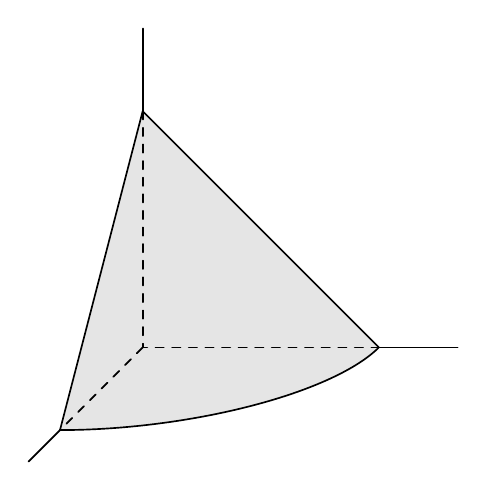
\begin{tikzpicture}[line width=.6pt,line join=round,line cap=round]
\coordinate (O) at (0,0);\coordinate (T) at (0,3);
\coordinate (R) at (3,0);\coordinate (L) at (-1.05,-1.05);
% Affine projection of a quarter circle in the horizontal plane.
\fill[gray!20] (T)--(L)--plot[domain=90:0,variable=\t,samples=91] ({3*cos(\t)-1.05*sin(\t)},{-1.05*sin(\t)})--cycle;
\draw (T)--(0,4.05);\draw (R)--(4,0);\draw (L)--(-1.45,-1.45);
\draw[dashed] (T)--(O)--(R);\draw[dashed] (O)--(L);
\draw (T)--(R);\draw (T)--(L);
\draw[domain=0:90,variable=\t,samples=91] plot ({3*cos(\t)-1.05*sin(\t)},{-1.05*sin(\t)});
\end{tikzpicture}
